
\section*{HS 2. feladat: Vízforraló üst acélfalának hőforgalma}
\addcontentsline{toc}{section}{HS 2. feladat}

\begin{tabular}{ | p{2cm} | p{14cm} | } 
	\hline
	Név & Kovács Bence \\ 
	\hline
	Szak &  Mechatronikai mérnöki alapszak\\
	\hline
	Félév & 2019/2020 II. (tavaszi) félév \\ 
	\hline
\end{tabular}
\vspace{0.5cm}


Egy vízforraló üst $d_1$ vastag acélfalának vízoldali hőfoka $T_1$, a falban kialakuló hőáramsűrüség $q_1$.

\noindent Adatok:    
($\lambda_{AC} = \SI{45.4}{\watt\per\meter\kelvin}$ ;
$\lambda_{\textit{vízkő}} = \SI{1,8}{\watt\per\meter\kelvin}$ ; 
$d_1 = \SI{20}{\milli\meter}$ ; 
$T_V = \SI{100}{\celsius} $ ; 
$q = \SI{60000}{\watt\per\meter\squared}$ ; )

\vspace{2mm}

\subsubsection*{Megoldás}


\subsubsection*{A) Határozza meg az üst füstgázoldali hőmérsékletét!}


Először felírjuk a hőáramsűrüségre vonatkozó egyenletet:

\begin{equation}
	 \dot{q} = \frac{\lambda_1}{\delta_1} (T_1 - T_2)
\end{equation}


Majd behelyettesítjük az értékeket:
\begin{equation}
60 \cdot \SI{1000}{\watt\per\meter\squared} =  \frac{\SI{45.4}{\watt\per\meter\kelvin}}{\SI{0.02}{\meter}} (T_{fg} - T_V)
\end{equation}

Mivel tudjuk, hogy $T_V = \SI{373.15}{\kelvin}$ , behelyettesítjül ezt is.
A zárójel felbontása után, a $T_2$-őt jobb oldalra rendezve az alábbi egyenletet kapjuk:

\begin{equation}
60 \cdot \SI{1000}{\watt\per\meter\squared}+  \frac{\SI{45.4}{\watt\per\meter\kelvin}}{\SI{0.02}{\meter}} \cdot \SI{373.15}{\kelvin}=  \frac{\SI{45.4}{\watt\per\meter\kelvin}}{\SI{0.02}{\meter}} \cdot T_2
\end{equation}

\begin{equation}
60 \cdot \SI{1000}{\watt\per\meter\squared} + \SI{847050.5}{\watt\per\meter\squared} = \SI{2270}{\watt\per\meter\squared} \cdot T_2
\end{equation}
\vspace{1mm}

Ebből $T_2$-őt ki tudjuk fejezni, ezzel meg is kapjuk az 'a' kérdésre a választ:

\begin{equation}
T_2 = \SI{399.58}{\kelvin} = \SI{126.43}{\celsius}
\end{equation}

\vspace{1mm}

\subsubsection*{B)  Határozza meg a két felület érintkezésnél kialakult hőmérsékletet, ha a vízoldalon $\SI{2}{\milli\meter}$ vastag vízkőréteg képződik és a fal két oldalán a hőmérséklet változatlan marad!}

\begin{equation}
	 \dot{q} = \frac{\lambda_1}{\delta_1} (T_1 - T_W)
\end{equation}

Majd felírjuk az $\dot{q}_1$ illetve $\dot{q}_2$-re vonatkozó egyenleteket. Mivel a vízkőréteg és a fal érintkezésénél nem ismerjük a hőmérsékletet, ezt paraméteresen $T_W$-vel fogjuk jelölni

\begin{equation}
	 \dot{q}_1 =  \frac{\SI{45.4}{\watt\per\meter\kelvin}}{\SI{0.02}{\meter}} (\SI{399.58}{\kelvin} - T_W)
\end{equation}


\begin{equation}
	 \dot{q}_2 =  \frac{\SI{1.8}{\watt\per\meter\kelvin}}{\SI{0.002}{\meter}} (T_W - \SI{373.15}{\kelvin})
\end{equation}

Majd egyszerűsítések után az alábbi két egyenletet kapjuk:

\begin{equation}     
     \dot{q}_1 = \SI{2270}{\watt\per\kelvin\meter\squared} \cdot (\SI{399.58}{\kelvin} - T_W)
\end{equation}


 \begin{equation}   
    \dot{q}_2 = \SI{900}{\watt\per\kelvin\meter\squared} \cdot (T_W - \SI{373.15}{\kelvin})
\end{equation}

A kapott egyenleteket egyenlővé tesszük egymással
    
\begin{equation}    
     \SI{2270}{\watt\per\kelvin\meter\squared} \cdot (\SI{399.58}{\kelvin}-T_2) =  \SI{900}{\watt\per\kelvin\meter\squared}(T_W-\SI{373.15}{\kelvin})
\end{equation}

Majd kiszámoljuk és rendezzük az egyenletet:

\begin{equation}
    \SI{1007}{\kelvin}-3 \cdot T_W = T_W-\SI{373.15}{\kelvin}
\end{equation}
        
$T_W$-t kifejezve az egyenletből megkapjuk a felületi érintkezésnél kialakul hőmérsékletet:

\begin{equation}
    T_W = \frac{\SI{1380}{\kelvin}}{3.52}} = \SI{392.08}{\kelvin} = \SI{118,93}{\celsius}
\end{equation}
    
\subsubsection*{C) Számítsa ki a falban lévő hőáramsűrüség változását!}
    
Behelyettesítve a kezdeti egyenletbe a kapott $T_W$ értéket, ki tudjuk számolni a hőáramsűrüséget is, amire a következőt kapjuk:
    
\begin{equation}
     \dot{q} = \SI{900}{\watt\per\K} \cdot (\SI{392.08}{\kelvin} - \SI{373.15}{\kelvin}) = \SI{17046}{\watt\per\meter\squared}
\end{equation}

Kivonva a kapott értéket az erdeteti feladat hőáramsűrüségéből, megkapjuk, hogy az eredeti feladathoz képest mennyivel változott ez az érték:

\begin{equation}
            60 \cdot 10^3 - 17046 =  \SI{42954}{\watt\per\meter\squared}
\end{equation}

\subsubsection*{A Feladat kiszámítása után ábrázoljuk a hőmérséklet-hely függvényeket:}

\begin{figure}[h]
	\centering
	\begin{subfigure}[b]{0.45\textwidth} 
		\centering
		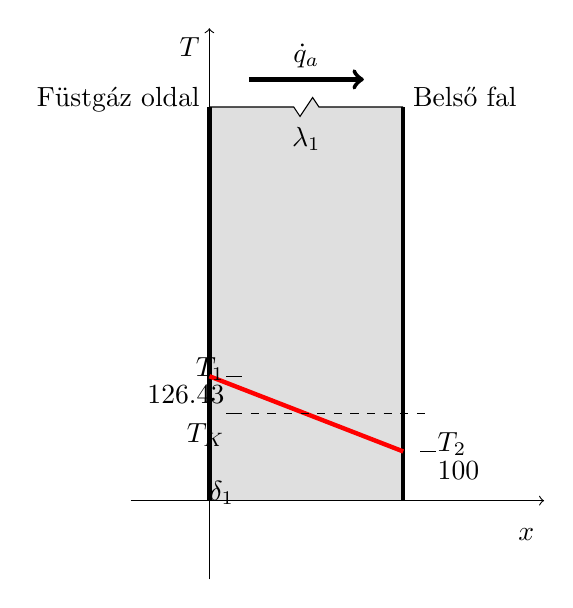
\begin{tikzpicture}
			\pgfmathsetmacro{\d}{16/6.5}
			\pgfmathsetmacro{\L}{5}
			\pgfmathsetmacro{\TA}{126.43/160*2}
			\pgfmathsetmacro{\TB}{100/160}
			\pgfmathsetmacro{\TK}{(\TA+\TB)/2}
			
			% Fal
			\fill[gray,opacity=0.25] (0,0) -- (0,\L) -- ({\d/2-0.16},\L) -- ({\d/2-0.08}, {\L-0.12}) -- ({\d/2+0.08}, {\L +0.12}) -- ({\d/2+0.16}, \L) -- (\d, \L) -- (\d, 0);
			\draw[] (0,\L) -- ({\d/2-0.16},\L) -- ({\d/2-0.08}, {\L-0.12}) -- ({\d/2+0.08}, {\L+0.12}) -- ({\d/2+0.16}, \L) -- (\d, \L);
			\draw[ultra thick] (0,0) -- (0,\L);
			\draw[ultra thick] (\d, 0) -- (\d, \L);
			
			% Feliratok
			\node[anchor=base east] at (0, \L) {Füstgáz oldal};
			\node[anchor=base west] at (\d, \L) {Belső fal};
			
			% Tengelyek
			\draw[->] (0,-1) -- (0,\L+1) node[anchor=north east]{$T$};
			\draw[->] (-1,0) -- (4.25,0) node[anchor=base east, shift={(0,-0.5)}]{$x$};
			
			% Hőáram és hőáramsűrűség
			\draw[->, ultra thick] (0.5,{\L+0.35}) -- ({\d/2},{\L+0.35}) node[anchor=south]{$\dot{q}_a$} -- ({\d - 0.5},{\L+0.35});
			
			% A hővezetési tényező
			\node[anchor=base] at ({\d/2},{\L-0.5}) {$\lambda_1$};
			
			% T(x)
			\draw[red, ultra thick] (0,\TA) -- (\d,\TB);
			
			% A delta_1 falvastagság
			\pgflength[xa=0, ya=0, xb=\d, yb=0, alim=0]{$\delta_1$};
			
			% A hőmérséklet értékek
			\draw (-0.1,\TA) -- (0.1,\TA);
			\node[anchor=base east] at (0,\TA) {$T_1$};
			\node[anchor=north east] at (0,\TA) {$\SI{126.43}{\celsius}$};
			
			\draw (-0.1+\d,\TB) -- (0.1+\d,\TB);
			\node[anchor=base west] at (\d,\TB) {$T_2$};
			\node[anchor=north west] at (\d,\TB) {$\SI{100}{\celsius}$};
			
			% A közepes hőmérséklet
			\draw[dashed] (0,\TK) -- (\d,\TK);
			\draw (-0.1,\TK) -- (0.1,\TK);
			\node[anchor=north east] at (0,\TK) {$T_K$};
			
		\end{tikzpicture}
		\caption{A hőmérséklet-hely függvény az a) esetben.}
	\end{subfigure}
	\begin{subfigure}[b]{0.45\textwidth}
		\centering
		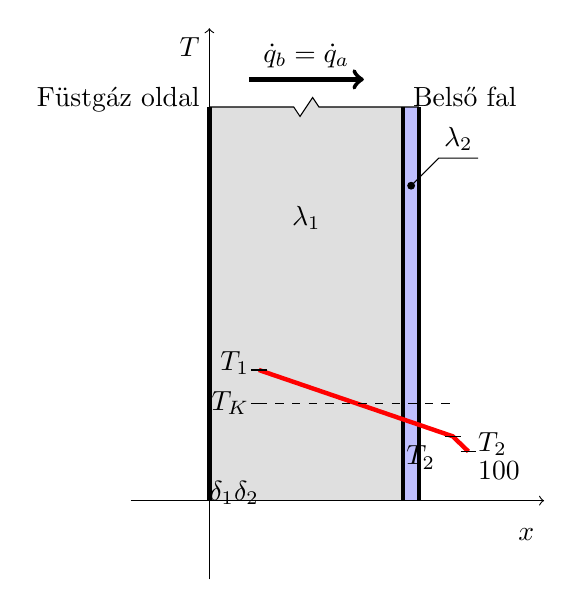
\begin{tikzpicture}
			\pgfmathsetmacro{\d}{16/6.5}
			\pgfmathsetmacro{\v}{1.2/6}
			\pgfmathsetmacro{\L}{5}
			\pgfmathsetmacro{\TA}{126.43/160*2.1}
			\pgfmathsetmacro{\TB}{118.93/160*1.1}
			\pgfmathsetmacro{\TC}{100/160}
			\pgfmathsetmacro{\TK}{(\TA+\TB)/2}
			
			% Fal
			\fill[gray,opacity=0.25] (0,0) -- (0,\L) -- ({\d/2-0.16},\L) -- ({\d/2-0.08}, {\L-0.12}) -- ({\d/2+0.08}, {\L +0.12}) -- ({\d/2+0.16}, \L) -- (\d, \L) -- (\d, 0);
			\fill[blue,opacity=0.25] (\d, \L) -- (\d, 0) -- (\d+\v, 0) -- (\d+\v, \L);
			\draw[] (0,\L) -- ({\d/2-0.16},\L) -- ({\d/2-0.08}, {\L-0.12}) -- ({\d/2+0.08}, {\L+0.12}) -- ({\d/2+0.16}, \L) -- (\d, \L) -- (\d+\v, \L);
			\draw[ultra thick] (0,0) -- (0,\L);
			\draw[ultra thick] (\d, 0) -- (\d, \L);
			\draw[ultra thick] (\d+\v, 0) -- (\d+\v, \L);
			
			% Feliratok
			\node[anchor=base east] at (0, \L) {Füstgáz oldal};
			\node[anchor=base west] at (\d, \L) {Belső fal};
			
			% Tengelyek
			\draw[->] (0,-1) -- (0,\L+1) node[anchor=north east]{$T$};
			\draw[->] (-1,0) -- (4.25,0) node[anchor=base east, shift={(0,-0.5)}]{$x$};
			
			% Hőáram és hőáramsűrűség
			\draw[->, ultra thick] (0.5,{\L+0.35}) -- ({\d/2},{\L+0.35}) node[anchor=south]{$\dot{q}_b = \dot{q}_a$} -- ({\d - 0.5},{\L+0.35});
			
			% A hővezetési tényező
			\node[anchor=base] at ({\d/2},{\L-1.5}) {$\lambda_1$};
			\node[anchor=base] at ({\d+\v+0.5},{\L-0.5}) {$\lambda_2$};
			\draw ({\d+\v+0.75},{\L-0.65}) -- ({\d+\v+0.25},{\L-0.65}) -- ({\d+\v/2},{\L-1});
			\fill[] ({\d+\v/2},{\L-1}) circle[radius=0.05];
			
			% A falvastagságok
			\pgflength[xa=0, ya=0, xb=\d, yb=0, alim=0]{$\delta_1$};
			\pgflength[xa=\d, ya=0, xb=\d+\v, yb=0, alim=0, a=0, belül=2]{$\delta_2$};
			
			% T(x)
			\draw[red, ultra thick] (0,\TA) -- (\d,\TB) -- (\d+\v,\TC);
			
			% Falhőmérsékletek
			\draw (-0.1,\TA) -- (0.1,\TA);
			\node[anchor=base east] at (0,\TA) {$T_1$};
			
			\draw (-0.1+\d,\TB) -- (0.1+\d,\TB);
			\node[anchor=north east] at (\d-0.1,\TB) {$T_2$};
			
			
			\draw (-0.1+\d+\v,\TC) -- (0.1+\d+\v,\TC);
			\node[anchor=base west] at (\d+\v,\TC) {$T_2$};
			\node[anchor=north west] at (\d+\v,\TC) {$\SI{100}{\celsius}$};
			
			% A közepes hőmérséklet
			\draw[dashed] (0,\TK) -- (\d,\TK);
			\draw (-0.1,\TK) -- (0.1,\TK);
			\node[anchor=east] at (0,\TK) {$T_K$};
			
		\end{tikzpicture}
		\caption{A hőmérséklet-hely függvény az b) esetben.}
	\end{subfigure}

\end{figure}

\pagebreak
